\section{Goodness-of-fitness} \label{sec:KS}
With the estimated parameters the sensors should be able to reconstruct the Idle and Active functions of the network and predict when or for how long the network will be idle. 
%JOHN: Do not refer to the Active, as it is out of scope here, i.e. we take it for granted.

In order to test if the reconstructed distributions (experimental distributions) fit with the empirical ones (obtained from the simulation) it is necessary the use of a Goodness-of-fitness test: the Kolmogorov-Smirnov test (\acs{K-S}). This validation test measures the deviation (D-value) of the empirical and experimental functions and the probability of null-hypothesis (P-value). The scientific community had determined that a null-hypothesis will be rejected if ${P<0.1}$.

In order to prove that the \acs{K-S} test is a good Goodness-of-fitness test for the proposed model, different tests had been developed following the same procedure for testing the \acs{MLE} in Section \ref{sec:MLE}.

During the testing of the \acs{K-S} test, different problems had been faced. At the beginning, the test had a high rate of failure, meaning that, that most of the time ${P<0.1}$. This meant that a review of the validation test should be done. Observing the procedure implemented by Marcello of the \acs{K-S} test in the NS framework, we realized that the failure was because the test was performed in both Uniform and Left-Pareto functions of the Idle distribution, and the higher number of samples gathered in the saturated part of the network ($[0 < t < \alpha_{bk}]$) affect the validation test. In order to have a better performance, we decided to apply the K-S test over just the long-tail of the mixture idle distribution and the results were clearly better as it is shown in Table \ref{table:KS}.

% JOHN: Theoretically, the test should not fail because of the mixed samples... It fails, though, because of the high uncertainty, or high noise, [write it as you like]. Anyway, the KS application to the truncated set of data does not guarantee, in advance, a better performance; we hope that it does - we do not prove it. So leave it open, and let the conclusion come after presenting the results.


\begin{table}[h!]
	\centering
	\begin{tabular}{ r | c | c }
		& Original \acs{K-S} & Modified \acs{K-S} \\ \hline
		Exponential Interarrival (mean: 1000 ms) & 8.76\% & 7\% \\ 
		Exponential Interarrival (mean: 100 ms) & 41.41\% & 12.56\% \\ 
		Constant Interarrival (mean: 100 ms) & 83.94\% & 100\% \\ 
		Uniform Interarrival (mean: 100 ms) & 37.56\% & 15.66\% \\ 
	\end{tabular}
	\caption{\acs{K-S} ${P(P<0.1)}$ - Uniform Packet Size (mean: 1550 bytes)}
	\label{table:KS}
\end{table}

From the table it can be observed how the probability of ${P<0.1}$ is better with the modified \acs{K-S}.
It can be observed how this modification in the validation test improves the performance for those cases with higher load. On the other hand we faced a problem with the constant interarrival case which need to be studied more in detail.

% JOHN: This problem is quite strange. I believe that there is no bug-error, so somehow the constant interrarival time distorts the fitting. Perhaps, we should use a more saturated network, in order to have shorter and longer idle periods, and then the fitting might be better. Since we have no good answer, do not present these results at all, until we fix it somehow :)

From the tests developed, the \acs{CDF} of the P-value has been extracted and compared between different tests. This is represented in Figure \ref{fig:cdf_p}.

As it can be observed, the distribution of the P-value is similar for all the active and idle distributions tested except for the constant interarrival case that we need still to study.

\begin{figure}[h!]
	\centering
	\subfloat[]{
		\label{fig:cdf_p_compare_active}
		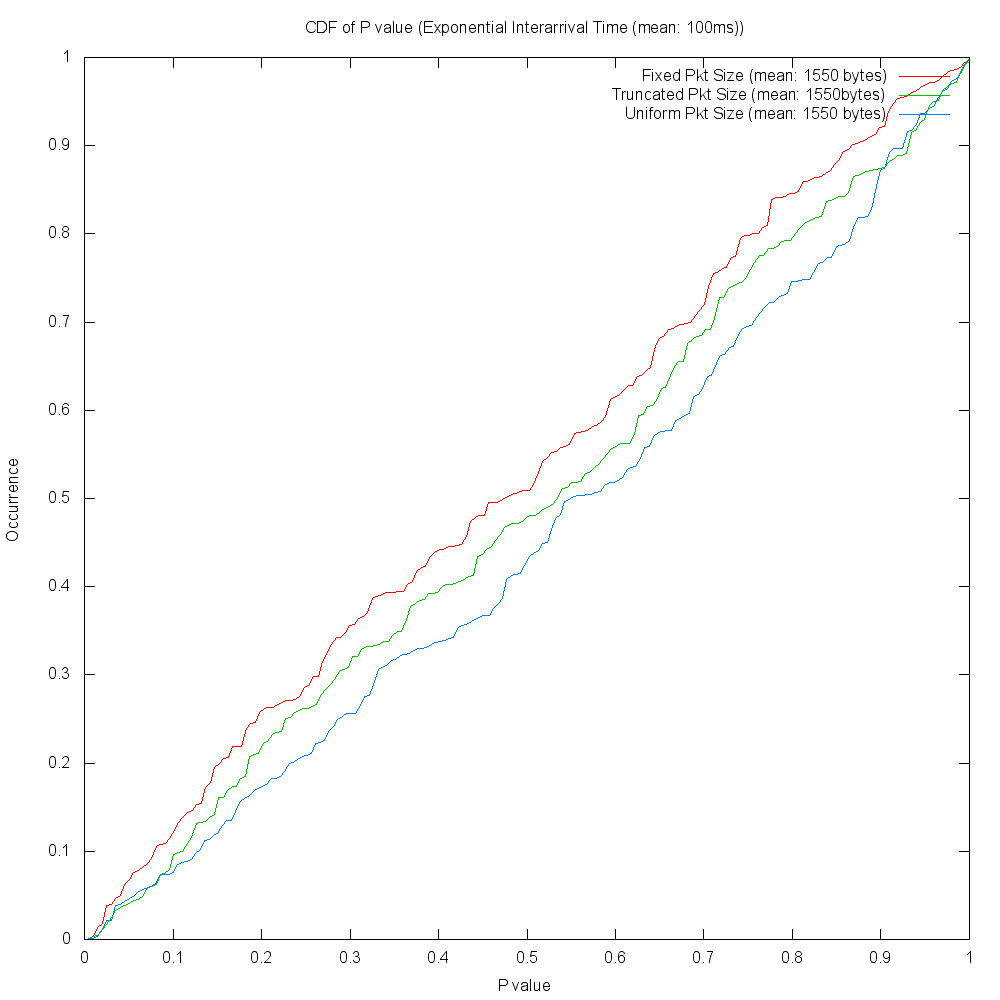
\includegraphics[width=0.45\textwidth]{images/results/GlobalView/KS/cdf_p/compare_active_exponential}
	}
	\subfloat[]{
		\label{fig:cdf_p_exp}
		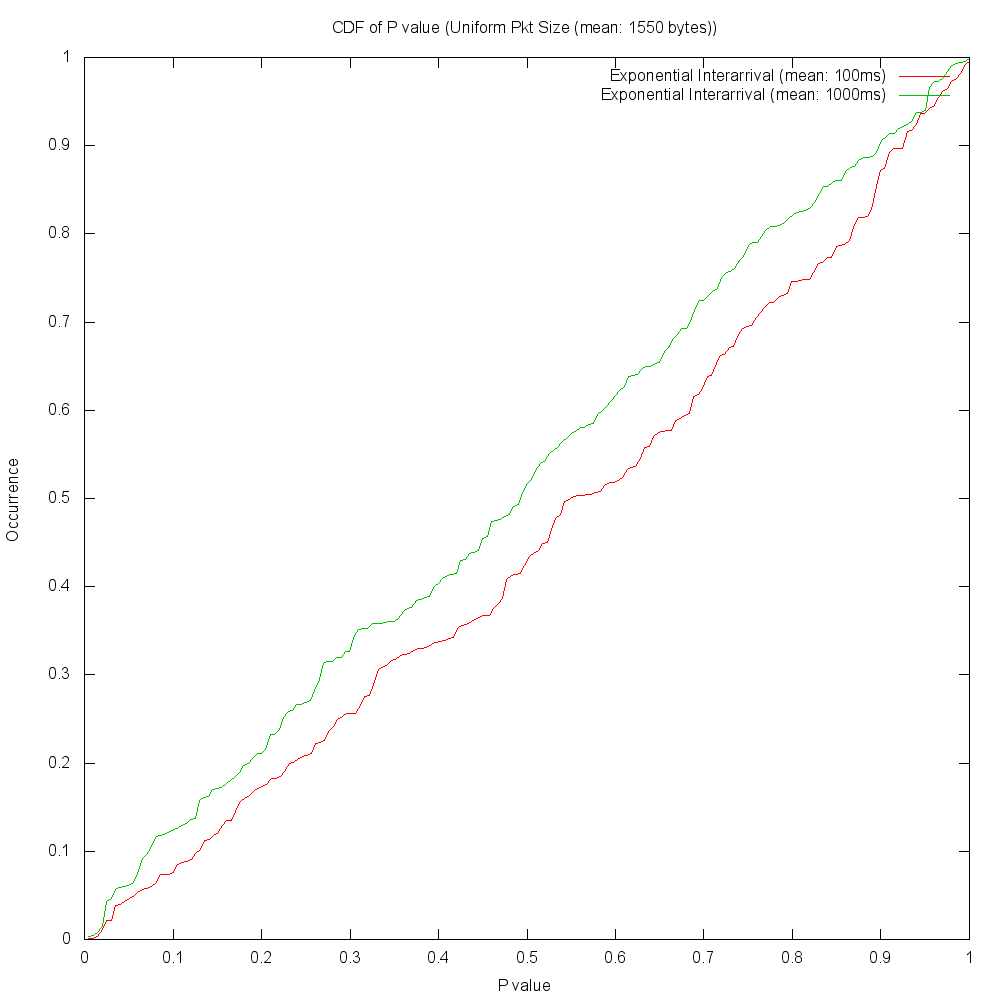
\includegraphics[width=0.45\textwidth]{images/results/GlobalView/KS/cdf_p/compare_exponential_interarrival}
	}
	\\
	\subfloat[]{
		\label{fig:cdf_p_fixed_size}
		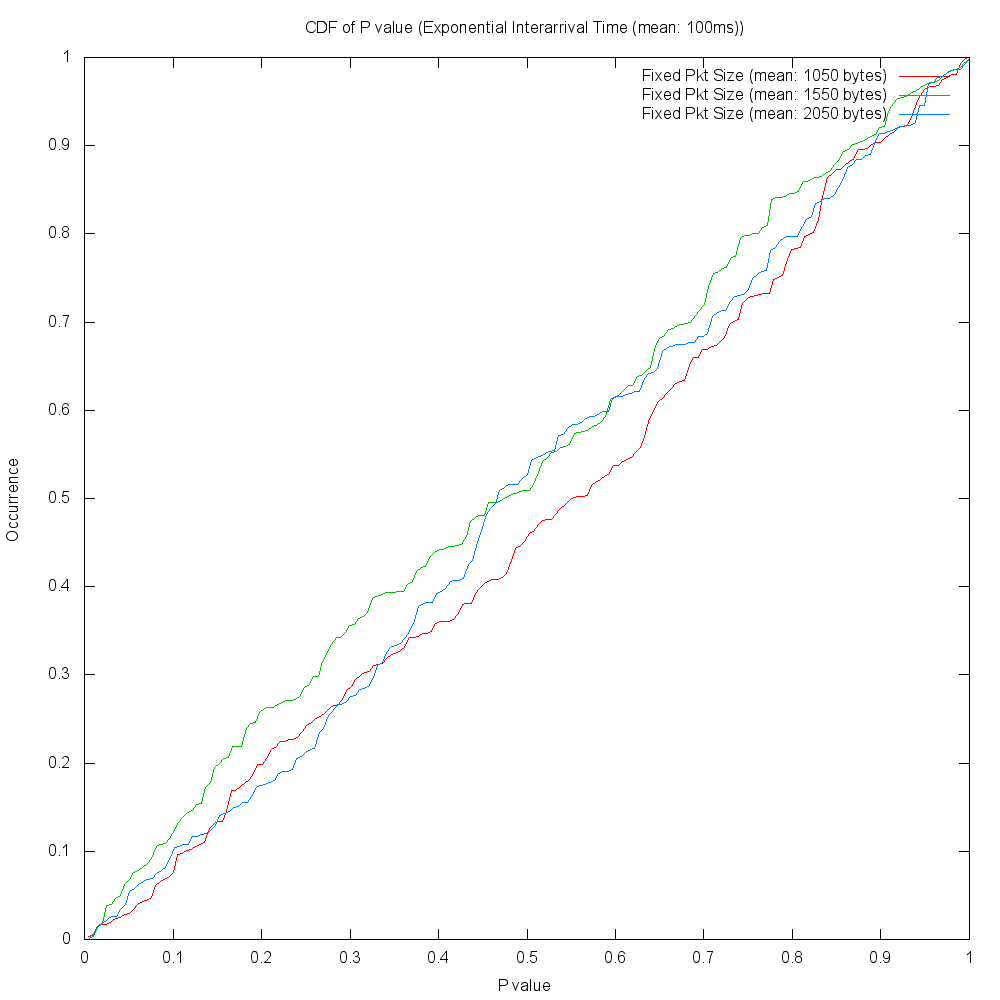
\includegraphics[width=0.45\textwidth]{images/results/GlobalView/KS/cdf_p/compare_fixed_size}
	}
	\subfloat[]{
		\label{fig:cdf_p_compare_idle}
		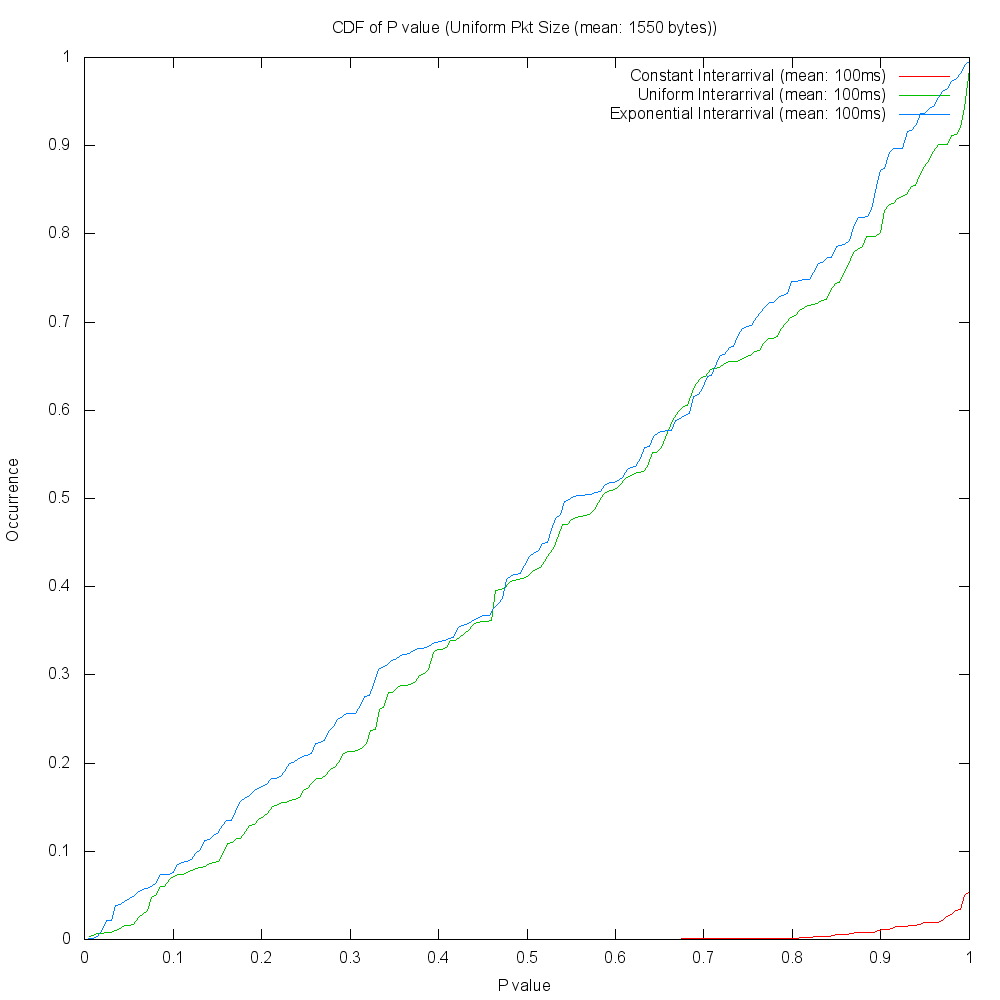
\includegraphics[width=0.45\textwidth]{images/results/GlobalView/KS/cdf_p/compare_idle_uniform}
	}
	\caption{\acs{CDF} of P value for different distributions}
	\label{fig:cdf_p}
\end{figure}

For those cases where ${P<<0.1}$, it is necessary to study if it is still possible to reconstruct the empirical distribution from the estimated parameters. From these cases, we observed that even for a really low P-value, the matching of the empirical and experimental distributions is almost perfect in almost all the cases studied as it is represented in Figure \ref{fig:ks_fail}. This makes us to reconsider if the \acs{K-S} test is the proper validation test in order to test the fitting between experimental and empirical functions for the proposed model.

% JOHN: I agree with the conclusion. For the moment, though, we do not apply a different test. We leave it OPEN for later...

\begin{figure}[h]
	\centering
	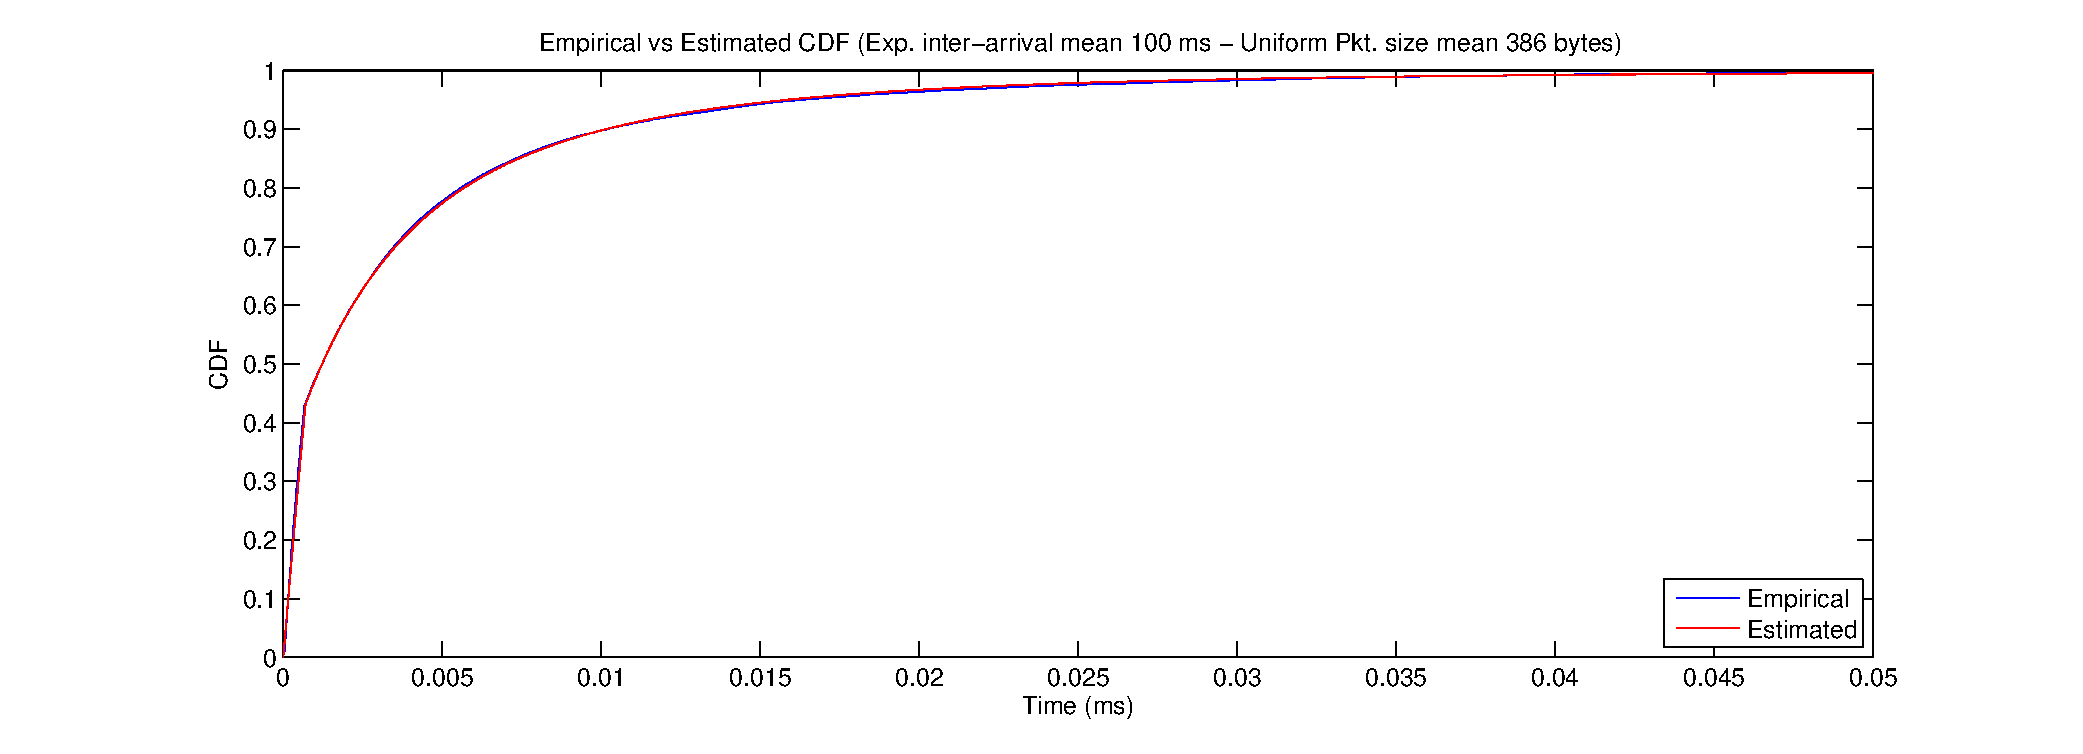
\includegraphics[scale=0.28, trim = 0mm 0mm 6mm 5mm, clip]{images/results/GlobalView/KS/ks_fail}
	\caption{Fitting of the \acs{CDF} of the experimental and empirical functions}
	\label{fig:ks_fail}
\end{figure}
